En el ambiente art\'istico \cite{Nishiguchi2017}, el trabajo desarrollado en
 Jap\'on por la Universidad de artes de Tokyo y la Universidad de Osaka, cuyo
 objetivo era brindar un comportamiento natural humano a un Robot Humanoide.
 Para cumplir esto utilizaron el conocimiento del director de escena Hirata,
 que dada la precisi\'on en sus instrucciones a los actores, facilita la
 traducci\'on de esas \'ordenes a las reglas para el robot humanoide, adem\'as,
 desarrollaron una interfaz de usuario para que el manejo del robot sea m\'as
 sencillo, ayudando a los principiantes, ya que proporcionan menos datos se
 puede obtener buenos resultados. 
\newpage 
 Como se puede observar en la figura
 ~\ref{fig:theatricalrob} el robot llego a desempe\~nar un amigo del
 personaje principal en la obra ``Night on the milky way train''
 (El tren nocturno de la v\'ia l\'actea) en un escenario real.


\begin{figure}[h]
\centering
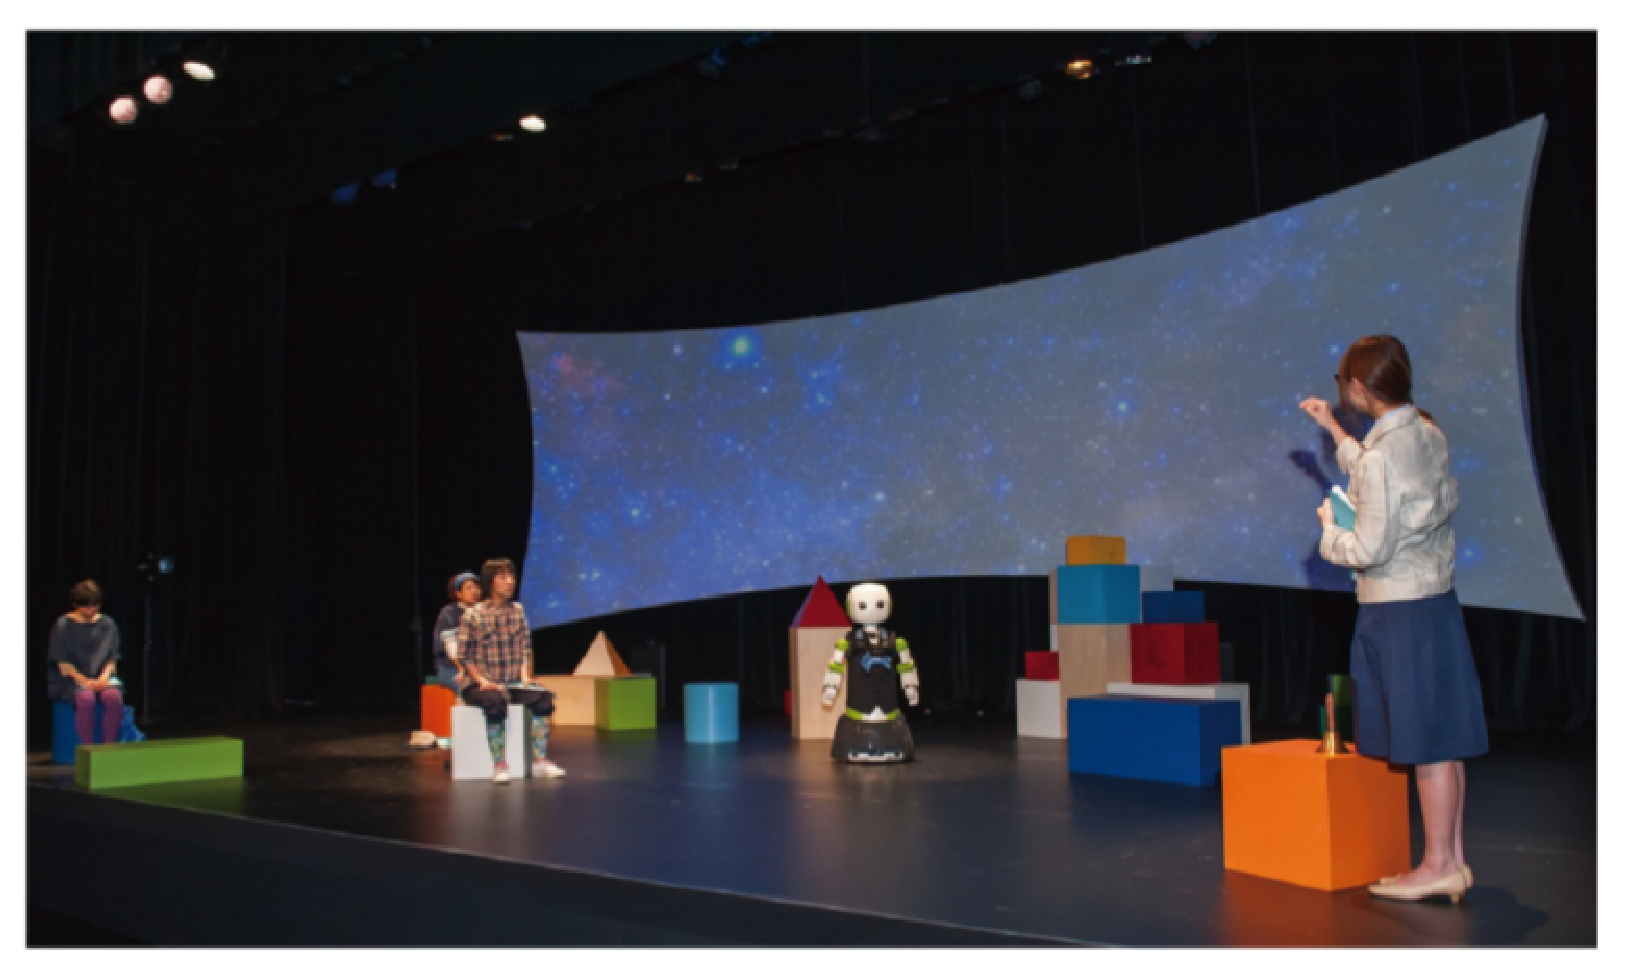
\includegraphics[width=0.8\columnwidth]{chap2/Imagenes/Theatrical.eps}
\caption{Robot humanoide actor en escenario real\cite{Nishiguchi2017}.}
\label{fig:theatricalrob}
\end{figure} 